%%%%%%%%%%%%%%%%%%%%%%%%%%%%%%%%%%%%%%%%%%%%%%%%%%%%%%%%%%%%%%%%%%%%%%%%%%%%%%%%
% IEEE FG 2027 submission (long paper: 8 pages + references, anonymised).
% Converted from ../main.tex (ACCV LNCS version). Build:  tectonic main.tex
%%%%%%%%%%%%%%%%%%%%%%%%%%%%%%%%%%%%%%%%%%%%%%%%%%%%%%%%%%%%%%%%%%%%%%%%%%%%%%%%
\PassOptionsToPackage{table,dvipsnames}{xcolor}
\documentclass[a4paper, 10pt, conference]{ieeeconf}
\usepackage{FG2027}

%\FGfinalcopy % *** Uncomment this line for the final submission

\IEEEoverridecommandlockouts
\overrideIEEEmargins

% tectonic (XeTeX) has no TU-encoded Times; force T1 so the body is set in Times
% as under pdflatex/Overleaf. No effect when compiled with pdflatex.
\usepackage{iftex}
\ifPDFTeX\else\usepackage[T1]{fontenc}\fi
\usepackage{graphicx}
\usepackage{booktabs}
\usepackage{amsmath,amssymb,amsfonts}
\usepackage{xcolor}
\usepackage{tikz}
\usetikzlibrary{arrows.meta,positioning,fit,calc,shapes.geometric}
\usepackage{adjustbox}
\usepackage{array}
\usepackage{multirow}
\usepackage[breaklinks,colorlinks,citecolor=blue,linkcolor=black,urlcolor=blue]{hyperref}

\setlength{\emergencystretch}{2em}
\newcommand{\tabtight}{\setlength{\tabcolsep}{3.5pt}\renewcommand{\arraystretch}{1.10}}

% ---- Convenience macros ----
\newcommand{\TDS}{\textsc{TDS}}

\def\FGPaperID{****} % *** Enter the FG2027 Paper ID here

\title{\LARGE \bf
Measuring and Mitigating Spatiotemporal Aliasing in Video Action Recognition:\\
A Cross-Architecture Analysis at Scale
}

% Camera-ready only (shown when \FGfinalcopy is active).
\author{\parbox{16cm}{\centering
    {\large Author Names}\\
    {\normalsize Affiliation}}
}

\begin{document}

\ifFGfinal
\thispagestyle{empty}
\pagestyle{empty}
\else
\author{Anonymous FG2027 submission\\ Paper ID \FGPaperID \\}
\pagestyle{plain}
\fi
\maketitle

\begin{abstract}
Temporal resolution in video-based human action and gesture recognition is usually treated as a fixed hyperparameter rather than a sampling constraint. We present a large-scale study of empirical classifier-evidence loss under temporal and spatial subsampling across 8 architectures and 8 datasets spanning sign-language gestures, hand--object interaction, driver behaviour, and fine-grained body movement (8,000 core evaluation configurations). Within this evaluated pool, aliasing sensitivity varies systematically across temporal aggregation designs: a state-space model and a divided-attention Transformer lose 2--4$\times$ less accuracy under frame reduction than standard Convolutional Neural Networks (CNNs), and a matched-evidence control that gives every model the same distinct frames confirms the advantage of divided attention. We introduce the \textbf{Temporal Demand Score (\TDS{})} to quantify accuracy loss under temporal subsampling; its dataset ranking is stable across architecture pools and metric definitions, and it identifies sign-language gestures and fine-grained gymnastics as the two most temporally demanding domains. In a cross-resolution evaluation, CNNs degrade at novel resolutions without fine-tuning, whereas Transformers natively maintain accuracy. Furthermore, latency profiling shows video state-space models are 4--8$\times$ slower than efficient Transformers. To optimize deployment, we demonstrate a \textbf{confidence-based adaptive frame cascade} that, under held-out calibration, halves the frame budget of the two sampling-robust architectures without accuracy loss on all 8 datasets. Finally, we provide a reproducibility package and an interactive visualization dashboard to enable aliasing-aware engineering design of human-observing AI systems.
\end{abstract}

% =========================================================
\section{Introduction}
\label{sec:intro}

Recognizing human gestures and actions from video underlies sign-language understanding, driver monitoring, healthcare, and behaviour analysis~\cite{5771372,10484402}. The field has evolved from 3D ConvNets and dual-pathway networks~\cite{tran2015c3d,carreira2017i3d,tran2018r2plus1d,wang2018nonlocal,feichtenhofer2019slowfast} to video Transformers and state-space models~\cite{bertasius2021timesformer,arnab2021vivit,liu2022videoswin,fan2021mvit,tong2022videomae,wang2023videomaev2,li2024videomamba}.

Despite this diversity, all models are evaluated using standardized sampling recipes (8--32 uniformly-sampled frames at fixed stride), treating temporal resolution as a static implementation detail. This assumption fails in real-world deployments where constraints on computational hardware, power usage, sensor capabilities, or communication bandwidth make dense sampling infeasible~\cite{lin2019tsm}. This leaves two fundamental questions unanswered: \emph{when} does temporal subsampling become destructive, and \emph{why} do different architectures respond differently? The question is most acute for human-centred recognition---sign language, driver monitoring, and fine-grained body movement---where the discriminative evidence is often a brief handshape transition or phase change rather than scene appearance.

\paragraph{Sampling perspective}
The Nyquist--Shannon theorem~\cite{shannon1949communication} motivates the intuition that undersampling can distort a temporal signal rather than merely compress it, a principle also relevant to perception~\cite{vanrullen2007wagon} and deep learning~\cite{zhang2019antialiased}. We use this as a conceptual guide, but introduce an empirical Temporal Demand Score (\TDS{}) metric that measures how much classifier evidence is lost under controlled subsampling, not literal spectral aliasing of the raw video signal.

\begin{figure}[t]
\centering
\begin{adjustbox}{max width=\columnwidth}
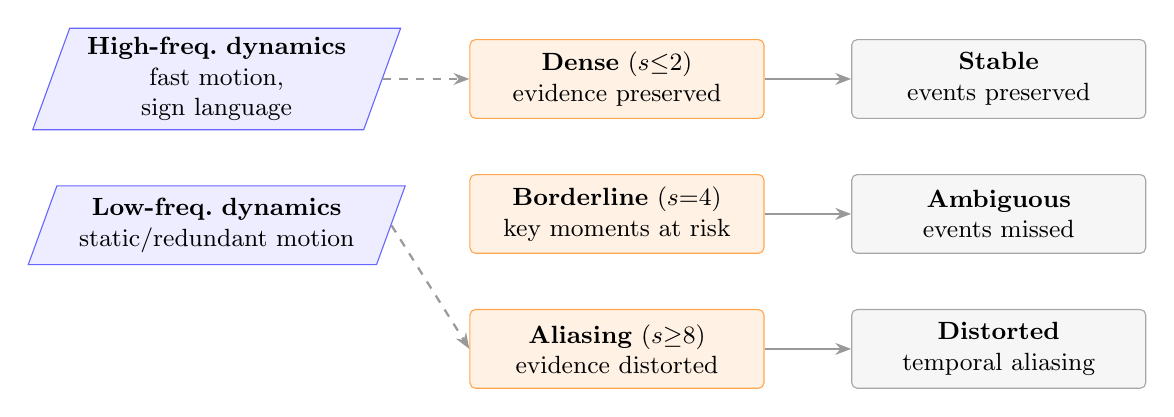
\begin{tikzpicture}[font=\small, node distance=7mm]
\tikzset{
  act/.style  ={draw, trapezium, trapezium left angle=70,
                trapezium right angle=110, align=center, minimum height=1.0cm, text width=3.5cm, fill=blue!7, draw=blue!60},
  samp/.style ={draw, rounded corners=2pt, align=center,
                minimum height=1.0cm, text width=3.5cm, fill=orange!10, draw=orange!70},
  obs/.style  ={draw, rounded corners=2pt, align=center,
                minimum height=1.0cm, text width=3.5cm, fill=gray!7, draw=gray!70},
  aI/.style={-{Stealth[length=2mm]},thick,dashed,draw=gray!80},
  aO/.style={-{Stealth[length=2mm]},thick,draw=gray!80}
}
\node (hf)[act]{\textbf{High-freq.\ dynamics}\\fast motion, sign language};
\node (lf)[act,below=of hf]{\textbf{Low-freq.\ dynamics}\\static/redundant motion};
\node (d)[samp,right=11mm of hf]{\textbf{Dense} ($s{\leq}2$)\\evidence preserved};
\node (n)[samp,below=of d]{\textbf{Borderline} ($s{=}4$)\\key moments at risk};
\node (a)[samp,below=of n]{\textbf{Aliasing} ($s{\geq}8$)\\evidence distorted};
\node (o1)[obs,right=11mm of d]{\textbf{Stable}\\events preserved};
\node (o2)[obs,below=of o1]{\textbf{Ambiguous}\\events missed};
\node (o3)[obs,below=of o2]{\textbf{Distorted}\\temporal aliasing};
\draw[aI](hf.east)--(d.west); \draw[aI](lf.east)--(a.west);
\draw[aO](d.east)--(o1.west); \draw[aO](n.east)--(o2.west); \draw[aO](a.east)--(o3.west);
\end{tikzpicture}
\end{adjustbox}
\caption{Temporal aliasing as empirical evidence loss: sparse sampling can miss or distort the frames a recognizer needs, especially for temporally localized actions.}
\label{fig:aliasing_concept}
\end{figure}

\paragraph{Contributions}
We conduct a systematic cross-architecture study of spatiotemporal aliasing in human action and gesture recognition:
\begin{enumerate}
\item \textbf{Temporal Demand Score (\TDS{})}: an architecture-averaged metric that measures a dataset's aliasing sensitivity. We demonstrate its utility by ranking 8 diverse datasets with leave-one-architecture-out analysis, architecture-family ablation (CNN-only, Transformer-only), and bootstrap confidence intervals checking ranking stability (Sec.~\ref{sec:results_tds}; supplementary material). 
% FineGym (55.9pp) rivals sign language (AUTSL, 53.0pp) as the highest-demand domain.
\item \textbf{Cross-architecture aliasing characterization}: 8,000 core evaluation
configurations show strong empirical architecture-level differences within our pool, with VideoMamba and TimeSformer losing 2--4$\times$ less accuracy under stride stress than CNNs and ViViT. A matched-evidence control that feeds every model the same distinct frames keeps TimeSformer first and agrees with this ordering under scarce evidence (Spearman $0.86$); this is an association, not a controlled temporal-module ablation (Sec.~\ref{sec:results_temporal}).
\item \textbf{Target-resolution fine-tuning}: Fine-tuning each model at the target spatial resolution closes the cross-resolution gap by up to 39pp for CNNs. In contrast, Transformers naturally maintain accuracy across different image sizes and require no retraining (Sec.~\ref{sec:results_spatial})
\item \textbf{Measured inference latency}: GPU latency characterization
across all 8 models $\times$ 5 target resolutions (bfloat16), enabling sampling-aware deployment budgeting (Sec.~\ref{sec:results_latency}).
\item \textbf{Practical illustration and reproducibility package}: as a low-cost downstream use of the temporal-sweep results above---rather than a new routing algorithm---a simple confidence-threshold cascade, calibrated on held-out data, matches dense-sampling accuracy with 57\% fewer frames on the Something-Something (SSv2) temporal dataset. We also provide a supplementary package containing a deterministic dashboard, evaluation scripts, and result tables; public code will be released after review (Sec.~\ref{sec:results_routing}).
\end{enumerate}

% =========================================================
\section{Related Work}
\label{sec:related}

\subsection{Video Recognition Architectures}

\textbf{CNN-based architectures.} 3D ConvNets learn spatiotemporal features end-to-end~\cite{tran2015c3d,carreira2017i3d}, while Non-local Networks introduce global self-attention~\cite{wang2018nonlocal}. Factorized variants such as R(2+1)D and MC3 improve optimization and efficiency~\cite{tran2018r2plus1d,tran2019video}; SlowFast processes two frame-rate streams simultaneously~\cite{feichtenhofer2019slowfast}.

\textbf{Transformer and SSM architectures.} Video Transformers extend patch-based recognition to time: TimeSformer uses divided space-time attention~\cite{bertasius2021timesformer}, ViViT uses factorized attention~\cite{arnab2021vivit}, and VideoMAE learns via masked patch reconstruction~\cite{tong2022videomae,wang2023videomaev2}. VideoMamba~\cite{li2024videomamba} brings selective state-space scanning~\cite{gu2023mamba,dao2024mamba2} to video. Prior robustness work benchmarks spatial and photometric corruptions~\cite{schiappa2023robustness}; we instead isolate temporal and spatial sampling effects across this architectural spectrum.

\subsection{Temporal Sampling and Adaptive Inference}

Efficient inference methods sample or process fewer frames. TSN and TSM define sparse-sampling recipes~\cite{wang2016tsn,lin2019tsm}; AdaFrame selects frames~\cite{wu2019adaframe}; AdaFocus crops regions~\cite{wang2021adafocus}; AR-Net adapts resolution~\cite{meng2020arnet}; and FrameExit uses confidence cascades~\cite{ghodrati2021frameexit}. Dataset-level temporal reasoning has been studied with shuffled frames~\cite{huang2018makes} and motion-only cues~\cite{sevilla2021only}. These works do not measure the accuracy cliff induced by controlled stride and coverage sweeps; our \TDS{} metric provides an architecture-averaged temporal-demand ranking.

\subsection{Sampling Theory in Deep Learning}

Sampling theory predicts that undersampling a signal below its highest temporal frequency creates aliasing~\cite{shannon1949communication}. Temporal aliasing is well documented in perception~\cite{vanrullen2007wagon}; in deep learning, strided operators can violate shift-invariance unless anti-aliased~\cite{zhang2019antialiased}. Frequency-domain analysis has been explored for action recognition~\cite{tran2014frequency}, but not as a large-scale cross-architecture stress test of modern video models.

% =========================================================
\section{Methodology}
\label{sec:method}

\begin{figure*}[t]
\centering
\resizebox{\textwidth}{!}{%
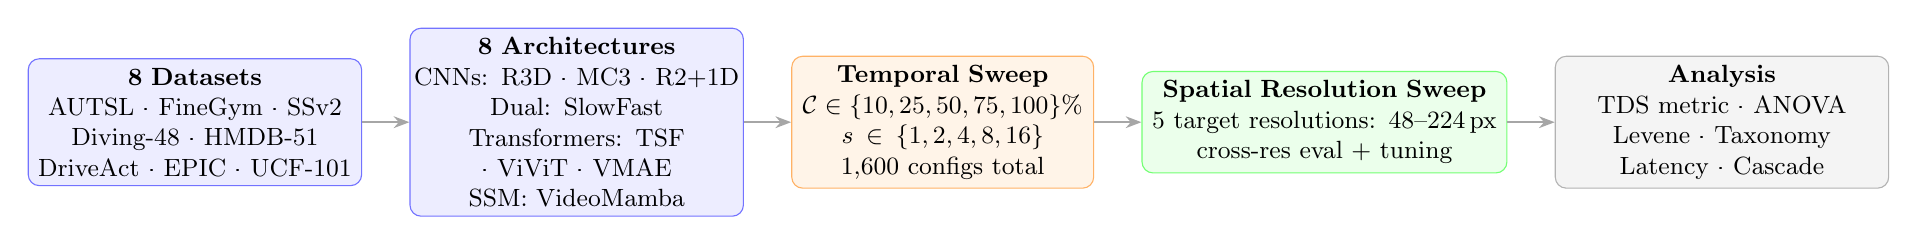
\begin{tikzpicture}[node distance=7mm,font=\small]
\tikzset{
  data/.style={draw,rounded corners,align=center,minimum height=8mm,text width=3.6cm,fill=blue!7,draw=blue!55},
  proc/.style={draw,rounded corners,align=center,minimum height=8mm,text width=3.6cm,fill=orange!9,draw=orange!60},
  p3/.style={draw,rounded corners,align=center,minimum height=8mm,text width=3.6cm,fill=green!8,draw=green!55},
  eval/.style={draw,rounded corners,align=center,minimum height=8mm,text width=4.0cm,fill=gray!9,draw=gray!60},
  arr/.style={-{Stealth[length=2mm]},thick,draw=gray!70}
}
\node(ds)[data,text width=4.0cm]{\textbf{8 Datasets}\\AUTSL \textperiodcentered{} FineGym \textperiodcentered{} SSv2\\Diving-48 \textperiodcentered{} HMDB-51\\DriveAct \textperiodcentered{} EPIC \textperiodcentered{} UCF-101};
\node(ar)[data,right=6mm of ds,text width=4.0cm]{\textbf{8 Architectures}\\\makebox[\linewidth]{CNNs: R3D \textperiodcentered{} MC3 \textperiodcentered{} R2+1D}\\Dual: SlowFast\\Transformers: TSF \textperiodcentered{} ViViT \textperiodcentered{} VMAE\\SSM: VideoMamba};
\node(e1)[proc,right=6mm of ar]{\textbf{Temporal Sweep}\\$\mathcal{C}\in\{10,25,50,75,100\}\%$\\$s\in\{1,2,4,8,16\}$\\1,600 configs total};
\node(e6)[p3,right=6mm of e1, text width=4.4cm]{\textbf{Spatial Resolution Sweep}\\5 target resolutions: 48--224\,px\\cross-res eval + tuning};
\node(an)[eval,right=6mm of e6]{\textbf{Analysis}\\TDS metric \textperiodcentered{} ANOVA\\Levene \textperiodcentered{} Taxonomy\\Latency \textperiodcentered{} Cascade};
\draw[arr](ds)--(ar); \draw[arr](ar)--(e1); \draw[arr](e1)--(e6); \draw[arr](e6)--(an);
\end{tikzpicture}}
\caption{Pipeline: the core factorial sweep uses 8 architectures $\times$ 8 datasets $\times$ 5 target resolutions (48--224px) $\times$ 5 coverages $\times$ 5 strides = \textbf{8,000 configurations}.}
\label{fig:pipeline}
\end{figure*}

\subsection{Datasets and Architectures}

Table~\ref{tab:datasets} summarizes the 8 datasets selected to span semantic domains, motion frequencies, and recording conditions. All depict human hand or body movement: isolated sign-language gestures (AUTSL), hand--object interaction (SSv2, EPIC-Kitchens), in-vehicle driver behaviour (DriveAct), fine-grained body movement (FineGym, Diving-48), and general human actions (HMDB-51, UCF-101). We evaluate 8 architectures from four families: (i) \textbf{3D CNNs}: R3D-18, MC3-18~\cite{tran2019video}, R(2+1)D-18~\cite{tran2018r2plus1d}; (ii) \textbf{dual-pathway}: SlowFast-R50~\cite{feichtenhofer2019slowfast}; (iii) \textbf{Transformers}: TimeSformer~\cite{bertasius2021timesformer}, ViViT~\cite{arnab2021vivit}, VideoMAE~\cite{tong2022videomae}; (iv) \textbf{SSM}: VideoMamba~\cite{li2024videomamba}. All models are fine-tuned from Kinetics-400 checkpoints using AdamW with cosine decay. We use fixed validation clip lists across models (approximately 20 clips/class, or all available clips for smaller classes); additional split, crop, seed, and frame-normalization details are in the supplementary material.

\begin{table}[t]
\centering
\caption{\TDS{} = mean accuracy drop (stride=1$\to$16, cov=100\%) per Eq.~\ref{eq:tds}, averaged over all 8 architectures ($n{=}8$). Sorted by \TDS{}. \textbf{Bold} = the two co-equal highest-demand domains (their relative order is leave-one-out sensitive; ranks 3--8 are stable under the supplementary robustness analysis).}
\label{tab:datasets}
\scriptsize\tabtight
\begin{tabular}{l r r l r r}
\toprule
Dataset & Classes & Videos & Domain & \TDS{} & $n$ \\
\midrule
FineGym~\cite{shao2020finegym}       &  97 & 1,600 & Fine-grained body motion & \textbf{55.9pp} & 8 \\
AUTSL~\cite{sincan2020autsl}         & 226 & 4,418 & Sign-language gestures & \textbf{53.0pp} & 8 \\
SSv2~\cite{goyal2017ssv2}            & 174 & 3,464 & Hand--object interaction & 27.6pp          & 8 \\
DriveAct~\cite{martin2019driveact}   &  33 &   448 & Driver behaviour & 21.9pp          & 8 \\
Diving-48~\cite{li2018diving48}      &  47 &   743 & Fine-grained body motion & 19.2pp          & 8 \\
HMDB-51~\cite{kuehne2011hmdb}        &  51 &   885 & General human actions & 16.6pp          & 8 \\
EPIC-Kitchens~\cite{damen2022epic}   &  89 & 1,020 & Egocentric hand--object &  9.7pp          & 8 \\
UCF-101~\cite{soomro2012ucf101}      & 101 & 2,020 & General human actions &  4.9pp          & 8 \\
\bottomrule
\end{tabular}
\end{table}

\subsection{Temporal Sampling Protocol}

We decouple \textit{temporal coverage} $\mathcal{C}$ (fraction of clip observed) from \textit{temporal stride} $s$ (sampling density), forming a 5$\times$5 grid: $\mathcal{C}\in\{10,25,50,75,100\}\%$ and $s\in\{1,2,4,8,16\}$. The temporal sweep at native resolution yields $8{\times}8{\times}25{=}\mathbf{1{,}600}$ model--dataset--configuration triples. Repeating this grid at the 5 target resolutions from 48--224px yields the \textbf{8,000} core configurations.

\paragraph{Coverage implementation}
Coverage is applied from the \emph{beginning} of each clip: the first $\lfloor T\cdot\mathcal{C}/100\rfloor$ frames form the candidate pool, and $s$ controls sampling density within that window. This simulates a sensor that observes only a leading fraction of the action and gives the sharpest measurement of how early the model has enough temporal context. Random window placement would confound temporal structure with missing-data effects; a 10\% random-window check on Something-Something (SSv2) gives qualitatively similar coverage effects (supplementary material).

\paragraph{Frame selection}
Every architecture consumes a fixed number of frames $B$: 8 for TimeSformer and VideoMamba, 16 for the 3D CNNs and VideoMAE, and 32 for SlowFast and ViViT. The strided candidate pool is resampled uniformly to $B$ frames, and if it holds fewer than $B$ frames the last one is repeated. Stride therefore alters the input once $\lceil \mathcal{C}T/100s\rceil<B$, \emph{i.e.}, when the stride no longer leaves $B$ distinct frames in the observed window, and the sweep measures the accuracy lost in this under-sampled regime. Because frame rates and clip lengths differ, a nominal stride corresponds to different physical rates: with frame rates measured from the files, the median interval between distinct sampled frames of a 16-frame model at $\mathcal{C}{=}100\%$ grows from 0.13\,s ($s{=}1$) to 0.48\,s ($s{=}16$) on AUTSL and from 0.40\,s to 0.62\,s on UCF-101 (per-dataset values in the supplementary material).

\subsection{Spatial Resolution Protocol}

\paragraph{Cross-resolution evaluation}
The resolution grid is 48, 96, 112, 160, and 224\,px. Native training resolution is 112px for CNNs and 224px for Transformers and VideoMamba.

\paragraph{Target-resolution fine-tuning}
For each model--dataset--resolution triple at the 5 target resolutions (48--224\,px), we fine-tune from the native-resolution checkpoint for 10 additional epochs. For Transformers and VideoMamba, positional embeddings are bicubically interpolated from the native grid to the target grid before fine-tuning. CNNs transfer directly, and SlowFast uses adaptive average pooling to support non-native resolutions.

\subsection{Temporal Demand Score (\texorpdfstring{\TDS{}}{TDS})}

We define \TDS{} as the architecture-averaged accuracy drop from stride=1 to stride=16:
\begin{equation}
  \begin{split}
  \TDS(\mathcal{D}) = \frac{1}{|\mathcal{M}|} \sum_{m\in\mathcal{M}} \bigl[&\mathrm{Acc}(m,\mathcal{D},s{=}1)\\[-4pt]
  &- \mathrm{Acc}(m,\mathcal{D},s{=}16)\bigr]^+
  \end{split}
  \label{eq:tds}
\end{equation}
where $[x]^+=\max(x,0)$, so a small negative drop (sparse sampling slightly outperforming dense sampling) contributes 0 rather than reducing the dataset score. We define feature collapse operationally as stride=1 Top-1 accuracy below 5\%; no model--dataset pair in the native-resolution \TDS{} computation met this criterion, so no entries are excluded and the ranking is unchanged. \TDS{} is architecture-pool averaged, but its dataset ranking is stable under leave-one-architecture-out, family ablations, and bootstrap resampling over our 8-model pool (Sec.~\ref{sec:results_tds}; supplementary material), suggesting it reflects dataset temporal structure rather than any single model. The ranking is also insensitive to the definition: dropping the clipping or integrating the whole stride curve leaves it unchanged (Spearman $1.00$), and normalising the drop by stride=1 accuracy or by headroom above chance exchanges only adjacent datasets ($0.95$).

\subsection{Statistical Analysis}

For each model-dataset pair, a two-way repeated-measures ANOVA with the clip as subject (all 25 cells score the same clips) decomposes accuracy variance into coverage, stride, and interaction components; we report partial $\eta^2$. Levene's test detects changes in per-class accuracy variance under sparse sampling. Post-hoc Welch tests with Bonferroni correction identify aliasing cliffs.

\subsection{Confidence-Based Routing}

Given temporal-sweep results at two operating points---cheap: cov=100\%/$s$=4; dense: cov=100\%/$s$=1---we route video $v$ by thresholding the maximum class probability of the cheap pass: \[ \hat{y}(v) = \begin{cases}
    \hat{y}_\text{cheap} & \text{if } \max_c\,p(c\mid v,s{=}4) > \tau \\
    \hat{y}_\text{dense} & \text{otherwise}
  \end{cases}
\] Cost is counted in acquired frames, normalised so that dense sampling costs 16 and stride-4 sampling costs 4; it measures acquisition and transmission rather than backbone compute, since each backbone still consumes its fixed input length. We select $\tau\in[0.10,\,0.95]$ on a calibration half of the validation split, subject to an average cost $\leq8$, and score it on the held-out half, repeating over 1000 stratified splits to obtain confidence intervals. No retraining is required; only the existing temporal-sweep inference is reused.

% =========================================================
\section{Results}
\label{sec:results}

\subsection{Temporal Demand Score Validates Architecture-Independent Ranking}
\label{sec:results_tds}

Figure~\ref{fig:tds_spectral}(a) ranks datasets by \TDS{}. \textbf{FineGym (55.9pp)} is the most important new finding in this dimension: fine-grained gymnastics phase transitions rival AUTSL sign language (53.0pp), showing that sport is not inherently low-\TDS{} when the label space requires sub-second phase discrimination. AUTSL requires dense sampling to discriminate fine handshape transitions, but FineGym's phase boundaries are comparably demanding. UCF-101 (4.9pp) is nearly appearance-driven: object identity and static scene cues often suffice.

Crucially, ranks 3--8 are stable under leave-one-architecture-out: removing any single architecture leaves SSv2, DriveAct, Diving-48, HMDB-51, EPIC-Kitchens, and UCF-101 in the same order. Only the \#1/\#2 position swaps when VideoMamba is removed, so we report FineGym and AUTSL as co-equal high-\TDS{} domains. This stability also holds for CNN-only, Transformer-only, and Transformer+SSM pools (Spearman $\rho\geq0.976$ against the full pool), while bootstrap resampling gives a FineGym$-$AUTSL 95\% CI of $[-4.6,\,+11.7]$pp, consistent with zero (supplementary material). Short clips reach the under-sampled regime more often, and the share of clips that do so at $s{=}16$ is rank-correlated with \TDS{} (Spearman $0.96$); clip length alone does not set the score, however, since AUTSL, SSv2, and DriveAct are all entirely in this regime at $s{=}16$ and still span 21.9--53.0pp.

\paragraph{Spectral validation}
Figure~\ref{fig:tds_spectral}(b) correlates optical-flow magnitude with per-class aliasing loss. AUTSL and DriveAct show the expected positive within-dataset trend: classes with more motion alias more. EPIC-Kitchens is near zero, suggesting that egocentric camera motion decouples raw flow from action-relevant demand. FineGym is inverted ($r=-0.475$, $p<0.0001$): high-flow gymnastics classes often remain visually distinctive from almost any frame, while low-flow held positions or balance corrections depend on brief key moments. Thus raw flow magnitude is only a partial proxy for temporal demand, especially when class identity hinges on a discrete event rather than sustained motion (Table~\ref{tab:spectral}).

\paragraph{The inversion generalizes beyond FineGym} A spectral check on all 8 datasets across 5 resolutions pairs whole-frame optical-flow cutoff frequency with empirical stride-sensitivity at the same resolution (40 points; supplementary material). The relationship is significantly \emph{negative} ($\rho=-0.63$, $p=1.1{\times}10^{-5}$): UCF-101 and HMDB-51 have high flow-derived cutoffs but low stride-sensitivity, while FineGym and AUTSL have the highest stride-sensitivity at lower cutoff frequencies. Thus whole-frame flow does not validate a literal Nyquist account; it shows that classifier-relevant evidence is often localized and diluted by bulk motion. A supplementary sliding-window diagnostic is more consistent with this evidence-localization view: per-class correct-class confidence concentration is positively associated with per-class aliasing loss (pooled Spearman $\rho=+0.26$ over a 6-architecture ensemble).

\begin{figure}[t]
  \centering
  \includegraphics[width=\columnwidth]{images/fig_tds_spectral.pdf}
  \caption{\textbf{(a)} \TDS{} ranking: mean accuracy drop from stride=1 to 16 averaged over all 8 architectures. FineGym and AUTSL are co-equal highest-demand domains (their order is leave-one-out sensitive); positions 3--8 are stable under leave-one-architecture-out. \textbf{(b)} Pearson correlation between optical-flow magnitude and per-class aliasing loss (red: $p<0.05$). AUTSL and SSv2 show a significant positive correlation; EPIC-Kitchens is near zero (camera motion confounds flow); FineGym is the strongest but inverted ($r=-0.475$): discrete-event classes alias more than sustained-motion ones.}
  \label{fig:tds_spectral}
\end{figure}

\begin{table}[t]
\centering
\caption{Spectral validation: Pearson $r$ between optical-flow magnitude and per-class aliasing loss. Flow alone partially explains temporal demand; camera-motion-heavy datasets (EPIC, UCF) show weak correlation.}
\label{tab:spectral}
\scriptsize\tabtight
\begin{adjustbox}{max width=\columnwidth}
\begin{tabular}{l r r c r}
\toprule
Dataset & Classes & Pearson $r$ & Significant & Interpretation \\
\midrule
FineGym       &  97 & $-0.475$ & \checkmark & Discrete-event classes alias more \\
DriveAct      &  33 & 0.327 & marginal   & Flow $\sim$ arm motion \\
AUTSL         & 226 & 0.285 & \checkmark & Flow $\sim$ hand speed \\
SSv2          & 174 & 0.184 & \checkmark & Causal/object motion \\
HMDB-51       &  51 & 0.180 & $\times$   & Mixed motion types \\
Diving-48     &  47 & 0.140 & $\times$   & Body rotation dominated \\
UCF-101       & 101 & 0.031 & $\times$   & Appearance dominates \\
EPIC-Kitchens &  89 & $-0.002$& $\times$ & Camera motion confounds \\
\bottomrule
\end{tabular}
\end{adjustbox}
\end{table}

\subsection{Cross-Architecture Temporal Aliasing}
\label{sec:results_temporal}

\paragraph{Attention type correlates with aliasing}
Table~\ref{tab:e1_full} shows stride=1 accuracy and stride=16 drop. The central observational finding is that aliasing aligns more with temporal aggregation design than with broad architecture family in this pool, although many architectural and training factors covary. The robust group is TimeSformer (divided attention, 10.3pp mean drop) and VideoMamba (SSM, 11.2pp). Both appear to preserve global temporal context under aggressive subsampling: TimeSformer via full-clip cross-frame attention, and VideoMamba via recurrent state accumulation.

VideoMamba's robustness is markedly \emph{bimodal}. It drops only 4.0pp on average over UCF-101, HMDB-51, EPIC-Kitchens, Diving-48, and DriveAct, which would make it the most robust model by a large margin if these were the only domains considered. But on the three highest-\TDS{} domains, VideoMamba suffers substantially: FineGym (40.0pp), AUTSL (16.0pp), and SSv2 (14.1pp). FineGym most clearly inverts the SSM-vs-Transformer ranking: TimeSformer drops 36.1pp vs.\ VideoMamba's 40.0pp, a 3.9pp gap favoring divided attention. The same direction holds on SSv2, while AUTSL is tied. We hypothesize that VideoMamba's running state smooths over high-frequency phase transitions, whereas TimeSformer can selectively attend to the most discriminative frames.

The SSv2 result extends beyond temporal frequency: SSv2 tests causal ordering (e.g., move object left then right), not just temporal density. SSM recurrence over skipped frames integrates corrupted order evidence, while appearance-driven UCF-101 remains stable. The fragile group comprises SlowFast (42.1pp), VideoMAE (32.8pp), ViViT (30.0pp), R2+1D (30.0pp), R3D-18 (29.7pp), and MC3-18 (22.6pp). ViViT is the key anomaly: a Transformer whose factorized attention remains vulnerable to frame dropout.

\paragraph{Matched-evidence control}
Because $B$ differs across architectures, models enter the under-sampled regime at different strides, and $B$ is itself rank-correlated with the mean drop of Table~\ref{tab:e1_full} (Spearman $0.85$). We therefore re-evaluate every architecture on the \emph{same} $k$ distinct frames at the same temporal positions, for $k\in\{1,2,4,8\}$, on all datasets except FineGym. The two ends of Table~\ref{tab:e1_full} persist: TimeSformer is the most accurate architecture at every $k\geq2$, by 4--11pp, and SlowFast the least accurate at $k\geq4$. Accuracy at matched evidence is positively associated with the ordering of Table~\ref{tab:e1_full} at every $k$ (Spearman $0.48$--$0.86$), most strongly under scarce evidence ($k{=}2$: $0.857$, $p{=}0.007$), and the accuracy lost between $k{=}8$ and $k{=}2$ is not associated with $B$ ($0.23$, $p{=}0.58$). The control also qualifies two readings of Table~\ref{tab:e1_full}. VideoMamba ranks third for $k\leq4$ but falls behind the CNNs at $k{=}8$, so its small drop partly reflects its 8-frame input. And the relative loss from $k{=}8$ to $k{=}2$ spans only 36--52\% across architectures, so the 2--4$\times$ gap combines input length with how efficiently each design uses the frames it receives (supplementary material).

\begin{figure*}[t]
  \centering
  \includegraphics[width=\textwidth]{images/fig_stride_curves.pdf}
  \caption{Accuracy vs.\ stride (cov=100\%) for three representative datasets. \textbf{AUTSL} (\TDS{}=53.0pp): TimeSformer and VideoMamba remain most stable; all other models cliff above stride=4. \textbf{SSv2} (\TDS{}=27.6pp): clear two-tier separation between robust (TSF, VMamba) and fragile models. \textbf{UCF-101} (\TDS{}=4.9pp): minimal sensitivity across all architectures. These three datasets span the full \TDS{} range.}
  \label{fig:aliasing_curves}
\end{figure*}

\begin{table*}[t]
\centering
\caption{Full temporal aliasing table: stride=1 accuracy (\%) / drop at stride=16 (pp), cov=100\%. Rows sorted by average drop across all 8 datasets.}
\label{tab:e1_full}
\scriptsize\tabtight
\begin{adjustbox}{max width=\textwidth}
\begin{tabular}{l @{\hskip4pt} cccccccc @{\hskip4pt} r}
\toprule
Model (family) & UCF-101 & SSv2 & HMDB-51 & Diving-48 & FineGym & AUTSL & DriveAct & EPIC-Kit. & Avg drop \\
\midrule
TimeSformer (div.\ attn) & 91.0/0.0 & 42.3/12.8 & 79.9/4.0 & 38.2/2.0 & 66.4/36.1 & 66.8/16.0 & 67.6/8.5 & 32.3/2.9 & \textbf{10.3pp} \\
VideoMamba (SSM)         & 88.4/0.8 & 43.9/14.1 & 69.8/3.6 & 36.5/4.6 & 73.3/40.0 & 65.6/16.0 & 57.6/9.2 & 28.3/1.6 & \textbf{11.2pp} \\
\midrule
MC3-18 (CNN-mix)  & 85.4/2.9  & 33.6/26.7 & 78.6/9.7  & 31.6/12.4 & 64.2/51.1 & 63.7/55.5 & 69.0/13.8 & 36.2/8.6  & 22.6pp \\
R3D-18 (CNN-3D)   & 81.2/6.0  & 37.1/28.2 & 80.3/21.1 & 28.8/16.0 & 71.5/61.4 & 75.0/68.5 & 68.3/23.9 & 37.2/12.7 & 29.7pp \\
R2+1D (CNN-sep.)  & 88.6/5.1  & 42.6/30.7 & 73.1/17.6 & 35.3/18.8 & 76.8/64.2 & 75.9/67.2 & 62.5/24.8 & 35.5/11.7 & 30.0pp \\
ViViT (fact.\ attn) & 94.3/5.2 & 38.3/30.6 & 80.2/19.4 & 53.0/36.3 & 69.9/55.2 & 74.6/62.1 & 67.4/20.3 & 32.9/11.1 & 30.0pp \\
VideoMAE (MAE)    & 95.4/3.5  & 52.4/34.4 & 84.0/20.2 & 48.6/23.4 & 78.0/67.8 & 79.6/61.2 & 73.9/40.8 & 37.7/10.8 & 32.8pp \\
SlowFast (dual)   & 87.6/15.4 & 49.5/43.0 & 79.3/37.4 & 50.5/39.7 & 78.2/71.5 & 82.3/77.6 & 72.5/33.7 & 39.4/18.5 & \textbf{42.1pp} \\
\bottomrule
\end{tabular}
\end{adjustbox}
\end{table*}

\paragraph{Architecture-specific failure modes}
SlowFast cliffs at stride 2$\to$4 because its fast and slow pathways are simultaneously starved; on FineGym it has the best base accuracy (78.2\%) but the largest drop (71.5pp). VideoMAE is spatially strong but temporally fragile: masked patch reconstruction does not train robustness to missing frames. VideoMamba's failures concentrate on high-frequency phase changes (FineGym), handshape transitions (AUTSL), and ordering-sensitive interactions (SSv2).

\paragraph{Cross-architecture sensitivity heatmap}
Figure~\ref{fig:heatmap} shows the stride-induced accuracy drop (stride=1 minus stride=16, in percentage points) at cov=100\%; larger values indicate stronger aliasing loss. Full per-model, per-dataset Top-1 accuracy heatmaps across coverage and stride are in the supplementary material.

\begin{figure}[t]
  \centering
  \includegraphics[width=\columnwidth]{images/fig_drop_heatmap.pdf}
  \caption{Cross-architecture aliasing-loss heatmap: accuracy drop (pp) from stride=1 to stride=16 at cov=100\%. Models are sorted top-to-bottom by increasing mean drop and datasets left-to-right by increasing \TDS{}.}
  \label{fig:heatmap}
\end{figure}

\subsection{Statistical Validation (ANOVA and Levene's Test)}
\label{sec:stats}

\paragraph{Effect sizes}
Table~\ref{tab:anova} reports partial $\eta^2$ from the repeated-measures ANOVA (mean$\pm$std over 8 datasets). Coverage is the larger factor on average ($0.29\pm0.16$ against $0.22\pm0.15$ for stride), and the coverage$\times$stride interaction is non-negligible ($0.06\pm0.08$, reaching $0.27$ on SlowFast/AUTSL). Stride effect size orders the architectures as in Table~\ref{tab:e1_full}, from VideoMamba ($0.10$) and TimeSformer ($0.12$) to SlowFast ($0.33$), a 3.2$\times$ difference. Per-dataset tables are provided in the supplementary material.

\begin{table}[t]
\centering
\caption{Repeated-measures ANOVA effect sizes (partial $\eta^2$, mean$\pm$std over 8 datasets; clip as subject). Stride separates robust from fragile architectures.}
\label{tab:anova}
\scriptsize\tabtight
\begin{tabular}{l ccc}
\toprule
Model & $\eta^2_\text{stride}$ & $\eta^2_\text{cov}$ & $\eta^2_\text{cov$\times$stride}$ \\
\midrule
VideoMamba     & $0.10 \pm 0.10$ & $0.25 \pm 0.19$ & $0.02 \pm 0.03$ \\
TimeSformer    & $0.12 \pm 0.11$ & $0.26 \pm 0.17$ & $0.02 \pm 0.03$ \\
MC3-18         & $0.20 \pm 0.16$ & $0.24 \pm 0.16$ & $0.07 \pm 0.09$ \\
R3D-18         & $0.23 \pm 0.14$ & $0.27 \pm 0.16$ & $0.07 \pm 0.09$ \\
R2+1D          & $0.24 \pm 0.14$ & $0.29 \pm 0.16$ & $0.08 \pm 0.09$ \\
ViViT          & $0.25 \pm 0.14$ & $0.29 \pm 0.15$ & $0.07 \pm 0.07$ \\
VideoMAE       & $0.26 \pm 0.15$ & $0.37 \pm 0.15$ & $0.08 \pm 0.08$ \\
SlowFast       & $0.33 \pm 0.14$ & $0.32 \pm 0.13$ & $0.11 \pm 0.10$ \\
\bottomrule
\end{tabular}
\end{table}

\paragraph{Variance inflation}
Levene's test finds a significant change in inter-class accuracy variance between stride 1 and stride 16 in 58\% of the 64 model--dataset pairs ($p<0.05$; 34\% after Bonferroni correction). The direction depends on the dataset. On HMDB-51 and UCF-101 variance inflates, most for VideoMAE/HMDB-51 ($2.0\times$) and R3D-18/HMDB-51 ($1.85\times$): sparse sampling breaks some classes while leaving others intact, a class-specific failure that mean accuracy hides. On the high-\TDS{} datasets variance shrinks instead, because accuracy falls for nearly all classes. TimeSformer and VideoMamba stay within $0.9$--$1.14\times$.

\subsection{Action Sensitivity Taxonomy}
\label{sec:taxonomy}

We classify each action class into three tiers by per-class aliasing loss (accuracy drop, stride=1$\to$16). Tier boundaries use the 33rd/67th percentiles.

\textbf{High-sensitivity} actions are temporally critical: in AUTSL, even the Low tier loses 38pp, confirming that the entire dataset requires dense sampling. In contrast, the UCF-101 Low tier is unaffected ($-0.3$pp): static, appearance-driven actions do not depend on sampling density. Table~\ref{tab:taxonomy_thresholds} reports per-dataset tier boundaries. The Low boundaries of AUTSL (46.7pp) and FineGym (50.4pp) lie above the High boundary of every other dataset ($\leq$31.8pp), confirming that sign language and fine-grained gymnastics form a distinct temporal-frequency regime.

\begin{table}[t]
\centering
\caption{Taxonomy tier boundaries: 33rd/67th percentiles of the per-class accuracy drop (pp, stride=1$\to$16, cov=100\%), with per-class drops averaged over the 8 architectures. Classes at or below the Low boundary alias minimally; above the High boundary they alias severely.}
\label{tab:taxonomy_thresholds}
\scriptsize\tabtight
\begin{tabular}{l r r r r}
\toprule
Dataset & Low $\leq$ & High $>$ & \# High & \# Low \\
\midrule
FineGym       & 50.4pp & 71.2pp & 33 & 32 \\
AUTSL         & 46.7pp & 57.3pp & 75 & 74 \\
SSv2          & 20.6pp & 31.8pp & 58 & 57 \\
DriveAct      & 14.0pp & 29.6pp & 11 & 11 \\
Diving-48     & 12.6pp & 22.4pp & 16 & 16 \\
HMDB-51       &  7.9pp & 20.2pp & 17 & 17 \\
EPIC-Kitchens &  0.0pp &  7.1pp & 30 & 11 \\
UCF-101       &  1.2pp &  6.2pp & 35 & 31 \\
\bottomrule
\end{tabular}
\end{table}

\textbf{Clip duration effect.} Counter-intuitively, shorter clips alias more severely (Pearson $r=-0.3$ to $-0.8$ across models): short clips have less temporal redundancy, so each missed frame removes a larger fraction of available evidence. On UCF-101 with R3D-18, clips $>$6s lose only 1.5pp at stride=16 vs.\ 16.2pp for clips $<$3s. This suggests that short clips should receive dense sampling irrespective of model confidence (details in the supplementary material).

\subsection{Spatial Resolution and Target-Resolution Fine-Tuning}
\label{sec:results_spatial}

\paragraph{Cross-resolution robustness}
Figure~\ref{fig:spatial} and Table~\ref{tab:spatial} show accuracy vs.\ input resolution for all 8 models on SSv2, evaluated \emph{without retraining}. A related empirical split appears in the spatial domain. CNNs (native 112px) degrade sharply at higher resolutions: R2+1D drops from 42.6\% at 112px to 20.8\% at 224px ($-21.8$pp). Transformers and VideoMamba (native 224px) stay within $\pm$7pp across 96--224px.

\begin{figure}[t]
  \centering
  \includegraphics[width=\columnwidth]{images/fig_spatial_resolution.pdf}
  \caption{Accuracy vs.\ input resolution on SSv2 (no retraining). CNNs (dashed, native=112px) degrade at off-native resolutions; Transformers and VideoMamba (solid, native=224px) stay within $\pm$7pp across 96--224px. Filled markers denote each model's native training resolution.}
  \label{fig:spatial}
\end{figure}

\begin{table}[t]
\centering
\caption{Spatial robustness on SSv2 (no retraining). Bold = native resolution. $\Delta_\text{max}$ = largest drop from native.}
\label{tab:spatial}
\scriptsize\tabtight
\begin{adjustbox}{max width=\columnwidth}
\begin{tabular}{l r rrrrr r}
\toprule
Model & Native & 96px & 112px & 160px & 224px & $\Delta_\text{max}$ \\
\midrule
R3D-18      & 112px & 35.9 & \textbf{37.1} & 30.3 & 17.2 & $-19.9$pp \\
MC3-18      & 112px & 32.4 & \textbf{33.6} & 27.8 & 14.8 & $-18.8$pp \\
R2+1D       & 112px & 40.1 & \textbf{42.6} & 36.2 & 20.8 & $-21.8$pp \\
SlowFast    & 224px & 27.7 & 32.4 & 45.7 & \textbf{49.5} & $-21.8$pp \\
\midrule
TimeSformer & 224px & 39.3 & 39.4 & 41.4 & \textbf{42.3} & $-3.0$pp \\
ViViT       & 224px & 36.4 & 37.1 & 38.1 & \textbf{38.3} & $-1.9$pp \\
VideoMAE    & 224px & 48.9 & 49.2 & 51.5 & \textbf{52.3} & $-3.4$pp \\
VideoMamba  & 224px & 37.5 & 39.3 & 42.5 & \textbf{43.9} & $-6.4$pp \\
\bottomrule
\end{tabular}
\end{adjustbox}
\end{table}

This spatial robustness pattern is similar across the 8 datasets (supplementary material). The largest off-native CNN drop in the 48--224px grid is 62.7pp (MC3-18 on DriveAct), whereas across 96--224px Transformers remain within $\pm$8pp on 7 of 8 datasets; EPIC-Kitchens is the exception.

\paragraph{Target-resolution fine-tuning recovers CNN performance}
Table~\ref{tab:p3} shows family-level averages after target-resolution tuning. CNNs recover sharply: at 224px, cross-resolution accuracy is 30.0\%, but fine-tuning reaches 69.2\% ($+39.2$pp). Transformers gain only at 160--224px; at 112px and below, the interpolated model without retraining is the better choice (50.3\% vs.\ 36.6\% at 48px), so they need no target-resolution tuning. Fine-tuning for the same 10 epochs at a model's \emph{native} resolution, where there is nothing to adapt, already gains about 7pp (CNNs at 112px, Transformers at 224px), so roughly 32pp of the CNN recovery is attributable to resolution adaptation itself.

\begin{table}[t]
\centering
\caption{Target-resolution fine-tuning: family-level mean accuracy (\%) averaged over all 8 datasets, without (---) and with (FT) fine-tuning from the native-resolution checkpoint for 10 epochs at each target spatial resolution. CNNs benefit by up to 39.2pp at off-native resolutions; Transformers are already near-native without retraining. FT columns average the available cells (57 of 64 at 48px, 63 at 112px).}
\label{tab:p3}
\scriptsize\tabtight
\begin{tabular}{l l ccccc}
\toprule
Family & & 48px & 96px & 112px & 160px & 224px \\
\midrule
\multirow{2}{*}{CNN (3 models)}      & --- & 24.6 & 58.5 & 60.2 & 51.8 & 30.0 \\
                                     & FT  & 49.3 & 64.9 & 67.7 & 68.5 & 69.2 \\
\midrule
\multirow{2}{*}{Transformer (3)}     & --- & 50.3 & 60.5 & 61.3 & 63.0 & 63.6 \\
                                     & FT  & 36.6 & 56.3 & 60.3 & 66.9 & 71.4 \\
\midrule
\multirow{2}{*}{SSM (VideoMamba)}    & --- & 17.7 & 39.7 & 41.4 & 46.2 & 49.1 \\
                                     & FT  & 31.5 & 41.2 & 45.1 & 54.5 & 59.7 \\
\midrule
\multirow{2}{*}{Dual-CNN (SlowFast)} & --- &  5.9 & 35.1 & 42.9 & 62.3 & 67.5 \\
                                     & FT  & 36.2 & 73.3 & 71.9 & 71.6 & 67.5 \\
\bottomrule
\end{tabular}
\end{table}

\subsection{Inference Latency and Deployment Budgeting}
\label{sec:results_latency}

Table~\ref{tab:latency} reports measured bfloat16 latency at batch 1. VideoMamba is slowest (8--15ms), 4--8$\times$ slower than VideoMAE (1.6--2.8ms) despite its SSM design. VideoMAE gives the best Transformer accuracy per ms, while CNN latency scales predictably with resolution.

\begin{table}[t]
\centering
\caption{Inference latency (ms/clip, bfloat16, batch=1, RTX PRO 6000 Blackwell). VideoMamba is 4--8$\times$ slower than VideoMAE despite being an SSM.}
\label{tab:latency}
\scriptsize\tabtight
\begin{tabular}{l ccccc}
\toprule
Model & 48px & 96px & 112px & 160px & 224px \\
\midrule
R3D-18      & 0.61 & 0.89 & 1.20 & 1.76 & 2.78 \\
MC3-18      & 0.61 & 0.85 & 1.18 & 1.84 & 3.15 \\
R2+1D       & 1.39 & 2.21 & 2.54 & 4.10 & 5.77 \\
SlowFast    & 3.09 & 3.11 & 3.11 & 3.13 & 4.10 \\
\midrule
TimeSformer & 3.25 & 3.24 & 3.20 & 3.20 & 4.30 \\
ViViT       & 1.55 & 1.77 & 1.99 & 3.19 & 6.35 \\
VideoMAE    & 1.57 & 1.79 & 1.78 & 1.92 & 2.82 \\
VideoMamba  & 8.06 & 8.15 & 8.18 & 10.03 & 15.44 \\
\bottomrule
\end{tabular}
\end{table}

\subsection{Confidence-Based Adaptive Routing}
\label{sec:results_routing}

Table~\ref{tab:routing} compares the confidence cascade at an average cost $\leq8$ frames (full curves in the supplementary material); we treat it as a deployment illustration rather than a separately trained method. AdaFocus~\cite{wang2021adafocus} and AR-Net~\cite{meng2020arnet} use ResNet-50 and are informational. Under held-out calibration the cascade reaches 42.2\% at 6.9 average frames and matches dense inference ($-0.03$pp, 95\% CI $[-1.07,+0.83]$) with 57\% fewer acquired frames. FrameExit~\cite{ghodrati2021frameexit} on the same backbone reaches 38.4\% at 9.9 frames; it counts frames processed by the backbone rather than frames acquired, so the two costs are indicative rather than strictly comparable.

\begin{figure}[t]
  \centering
  \includegraphics[width=\columnwidth]{images/fig_cascade.pdf}
  \caption{Confidence cascade on SSv2: accuracy vs.\ average frames as $\tau$ sweeps between stride-4 (cheap) and stride-1 (dense) inference, with the fixed operating points and the per-video oracle as references.}
  \label{fig:routing}
\end{figure}

\begin{table}[t]
\centering
\caption{Routing comparison on SSv2 at avg $\leq$8 frames. The cascade (ours, held-out calibration) is compared with its own fixed operating points on TimeSformer; cost is in acquired frames (stride 1 = 16, stride 4 = 4). FrameExit uses the same backbone but counts processed frames. AdaFocus/AR-Net use a different backbone (ResNet-50) and are reported only as context for absolute numbers reported in their respective papers, not as a controlled comparison.}
\label{tab:routing}
\scriptsize\tabtight
\begin{tabular}{l c c c}
\toprule
Method & Avg frames & SSv2 Top-1 & Backbone \\
\midrule
\multicolumn{4}{l}{\textit{Informational only: different backbone}} \\
AdaFocus~\cite{wang2021adafocus} & 8.0 & 54.7\% & ResNet-50 \\
AR-Net~\cite{meng2020arnet}      & 8.0 & 48.6\% & ResNet-50 \\
\midrule
\multicolumn{4}{l}{\textit{Same TimeSformer backbone}} \\
Oracle upper bound      & ---  & 47.3\% & TimeSformer \\
Stride 1 (dense)        & 16.0 & 42.3\% & TimeSformer \\
\textbf{Cascade (ours)} & \textbf{6.9} & \textbf{42.2\%} & TimeSformer \\
Stride 4 (cheap)        & 4.0  & 41.6\% & TimeSformer \\
FrameExit~\cite{ghodrati2021frameexit} & 9.9 & 38.4\% & TimeSformer \\
\bottomrule
\end{tabular}
\end{table}

For the two sampling-robust architectures the result holds on all 8 datasets: the held-out cascade stays within the confidence interval of dense accuracy everywhere, for TimeSformer (mean $-0.06$pp, 4.7--7.6 average frames) and for VideoMamba (mean $-0.23$pp, 5.0--7.3 frames). The benefit is architecture-dependent, as the temporal results predict: over all 64 model--dataset pairs the cascade costs 3.1pp on average at 6.7 frames, most for SlowFast ($-10.7$pp) and on FineGym, where stride-4 inference is itself degraded. Confidence routing is therefore appropriate for sampling-robust backbones rather than a universal substitute for dense sampling.

% =========================================================
\section{Discussion}
\label{sec:discussion}

\paragraph{Architecture and sampling}
Within our evaluated pool, the robust temporal group combines global divided attention (TimeSformer) or recurrent state integration (VideoMamba), while the fragile group includes CNNs and factorized-attention Transformers. VideoMamba remains bimodal: it is nearly flat on low-\TDS{} datasets but still aliases on FineGym, AUTSL, and SSv2, where brief phase changes, handshape transitions, or causal order matter. Spatial robustness follows a related but distinct pattern: patch-token Transformers are resolution-stable, whereas CNNs require target-resolution fine-tuning; ViViT's spatial robustness despite temporal fragility separates tokenization effects from temporal aggregation effects.

\paragraph{Spatial robustness}
The spatial results suggest that temporal and spatial robustness share some architectural ingredients but are not identical. CNNs' strided filters are tied to the spatial scale seen during training, which explains the sharp off-resolution degradation and the large recovery from target-resolution fine-tuning. Transformers remain stable across most resolutions because patch tokenization and global aggregation tolerate scale shifts, yet ViViT shows that this spatial invariance does not guarantee temporal robustness. VideoMamba again sits between these regimes: stable on some datasets, but less reliable on cluttered egocentric or in-vehicle scenes.

\paragraph{Deployment implications}
Resolution, latency, and sampling density should be searched jointly rather than treated as independent knobs. High-\TDS{} domains require stride$\leq$2, moderate-\TDS{} domains tolerate stride$\leq$4, and low-\TDS{} domains tolerate stride up to 16. Target-resolution tuning makes CNN resolution a cost dial; TimeSformer routing at 6.9 frames approaches dense R2+1D on SSv2 (42.2\% vs.\ 42.6\%). Training-time exposure also mitigates temporal loss: fine-tuning with randomly drawn coverage and stride on AUTSL recovers 28\% (TimeSformer) and 37\% (R3D-18, whose stride-16 accuracy rises from 6.5\% to 31.9\%) of the stride-16 drop, at a cost of 3.3 and 9.9pp of dense accuracy (supplementary material). For gesture and body-movement analysis in particular, sign language and fine-grained gymnastics are the two highest-demand domains: such systems should budget for dense sampling and select backbones by accuracy per frame rather than by dense-sampling accuracy alone. These trade-offs are deployment-relevant because a model that is slightly less accurate at dense sampling can become preferable once resolution, stride, and hardware latency are optimized together.

This also changes how one should read fixed-recipe video benchmarks. A single native-resolution, fixed-stride number can hide the fact that two models exchange rank once the temporal budget or input resolution changes. The dashboard and tables therefore expose operating points rather than only peak accuracy, making the sampling constraint explicit.

\paragraph{Limitations}
Our architecture analysis is observational: temporal aggregation design covaries with tokenization, pretraining objective, capacity, and optimization recipe, so we report empirical associations rather than a controlled causal mechanism. A stronger test would swap temporal modules inside a shared backbone while holding training and capacity fixed. The Nyquist framing is conceptual: whole-frame flow is inversely related to stride-sensitivity, while temporal concentration of correct-class confidence is positively associated with per-class aliasing (pooled Spearman $\rho=+0.26$; supplementary material). The matched-evidence control excludes FineGym and feeds large-$B$ models fewer frames than they were trained on. Latency is measured on a single GPU.

% =========================================================
\section{Conclusion}
\label{sec:conclusion}

We present a large-scale cross-architecture study of spatiotemporal aliasing in human action and gesture recognition. Across 8 architectures, 8 datasets, and 8,000 configurations, aliasing shows a strong empirical association with temporal aggregation design, with ViViT showing that Transformers are not automatically temporally robust. The \TDS{} metric identifies FineGym and AUTSL as co-equal high-demand domains, establishing fine-grained sport as a high-aliasing regime. VideoMamba is robust but bimodal and slow on GPU; target-resolution fine-tuning closes the CNN resolution gap by up to 39pp; and a held-out-calibrated confidence cascade halves the frame budget of TimeSformer and VideoMamba without accuracy loss. These results are useful beyond ranking models: they indicate when computation should be spent on denser temporal evidence, when frames can be removed with little cost, and when poor accuracy is caused by a sampling mismatch rather than by the recognizer alone. Reporting accuracy over stride, coverage, and resolution, therefore, gives practitioners a way to check whether an activity model has actually seen enough time to justify its prediction.

\section*{ETHICAL IMPACT STATEMENT}
This study evaluates existing recognition models on publicly available datasets and collects no new data from human subjects. Several of the datasets depict identifiable people, including sign-language signers and in-vehicle drivers; we use them under their original licences, only for action classification, and perform no identity or attribute recognition. Activity recognition can be misused for surveillance or intrusive monitoring, and our findings on how far temporal sampling can be reduced could lower the cost of such systems. We also show that sparse sampling degrades accuracy unevenly across action classes, so reducing frame budgets may affect some signers, gestures, or activities more than others; per-class evaluation is advisable before deployment. All experiments are inference or short fine-tuning runs, and the released results allow others to reuse them without repeating the computation.

{\small
\bibliographystyle{ieee}
\bibliography{main}
}

\end{document}
